\documentclass[12pt,a4paper]{article}

\usepackage[a4paper,text={16.5cm,25.2cm},centering]{geometry}
\usepackage{lmodern}
\usepackage{amssymb,amsmath}
\usepackage{bm}
\usepackage{graphicx}
\usepackage{microtype}
\usepackage{hyperref}
\usepackage{minted}
\setlength{\parindent}{0pt}
\setlength{\parskip}{1.2ex}

\hypersetup
       {   pdfauthor = {  },
           pdftitle={  },
           colorlinks=TRUE,
           linkcolor=black,
           citecolor=blue,
           urlcolor=blue
       }






\begin{document}



\section{Porazdelitvena funkcija za N(0, 1)}
Tina Brdnik

\subsection{Opis naloge}
Naloga obravnava porazdelitveno funkcijo standardne normalne porazdelitve N(0,1), ki je definirana kot:

\[
F(x) = \frac{1}{\sqrt{2\pi}} \int_{-\infty}^x e^{-t^2/2}\,dt
\]
Ta funkcija podaja verjetnost, da je slučajna spremenljivka z normalno porazdelitvijo manjša ali enaka vrednosti x.

\subsection{Opis rešitve}
Implementacija algoritma poteka v več korakih:

\begin{itemize}
\item[1. ] Numerična integracija z Simpsonovim pravilom  

\end{itemize}
Uporabimo sestavljeno Simpsonovo pravilo za izračun določenega integrala funkcije gostote normalne porazdelitve. To pravilo združuje vrednosti funkcije v krajiščih in središčih podintervalov ter zagotavlja visoko natančnost.

\begin{itemize}
\item[2. ] Posebni primeri  

\end{itemize}
Za $x = 0$ lahko rezultat podamo neposredno kot $F(0) = 0.5$. Za zelo velike vrednosti $|x|$ uporabimo asimptotsko aproksimacijo repa normalne porazdelitve, da se izognemo nepotrebnemu računanju na daljših intervalih.

\begin{itemize}
\item[3. ] Simetrija funkcije  

\end{itemize}
Ker velja $F(-x) = 1 - F(x)$, za negativne vrednosti $x$ izračunamo rezultat prek pozitivnega argumenta. Na ta način izkoristimo lastnosti normalne porazdelitve in poenostavimo izračun.

\begin{itemize}
\item[4. ] Kombinacija metod  

\end{itemize}
Za $x > 0$ integral izračunamo z uporabo Simpsonovega pravila na intervalu $[0,x]$, pri tem pa dodamo začetno vrednost $0.5$, ki ustreza $F(0)$. Tako dobimo splošno funkcijo $F(x)$, ki vrača približek porazdelitvene funkcije standardne normale.


\subsection{Rezultati}
Funkcijo $F(x)$ smo primerjali z referenčno rešitvijo, izračunano s pomočjo funkcije 'erf'. Na spodnjem grafu sta prikazani obe krivulji, ki se praktično popolnoma prekrivata. Izračunali smo tudi delež točk, kjer je bila napaka manjša od dovoljene tolerance, in dobili rezultat 100 \%.


\begin{minted}[texcomments = true, mathescape, fontsize=\small, xleftmargin=0.5em]{julia}
include("demo.jl")
using .Naloga2
plt, pct = demo_F()
display(plt)
\end{minted}
\begin{minted}[texcomments = true, mathescape, fontsize=\small, xleftmargin=0.5em, frame = leftline]{text}
Pravilnih izračunov: 100.0 %
\end{minted}
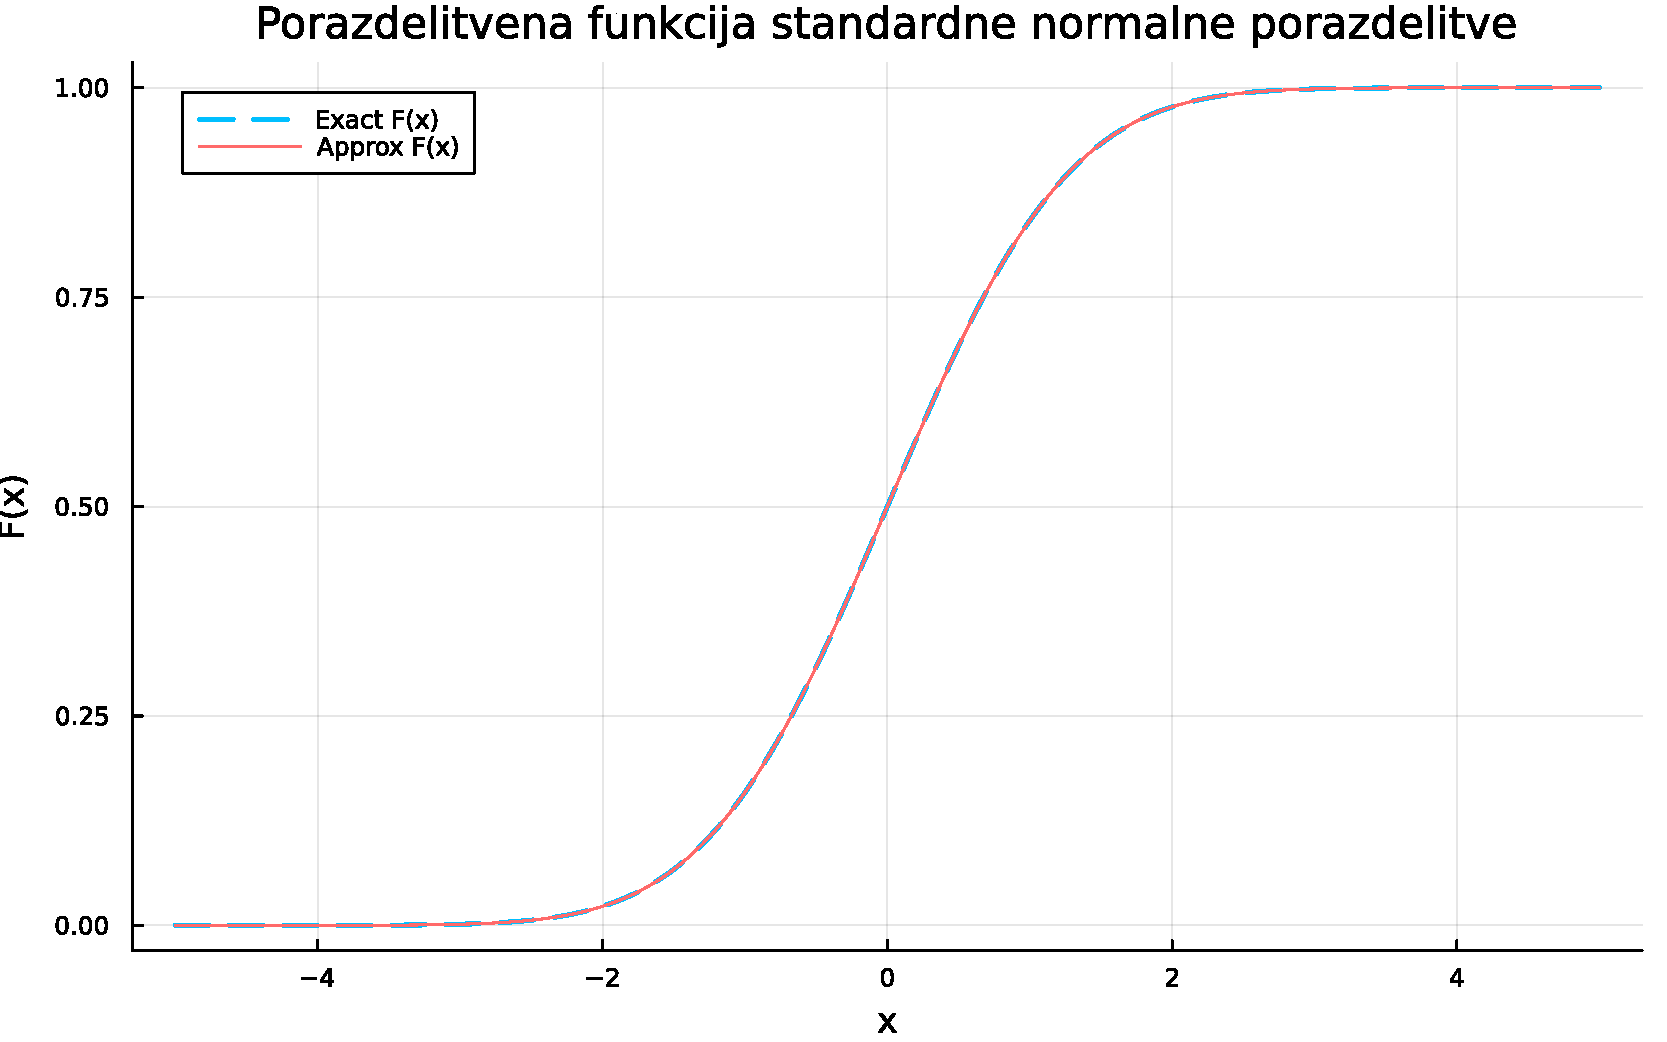
\includegraphics[width=\linewidth]{jl_x9oW6m/porocilo1_0_1.pdf}


\end{document}
